\documentclass[a4paper,ngerman,landscape]{scrartcl}

\usepackage[utf8]{inputenc}

\usepackage[ngerman]{babel}
\usepackage{hyperref}

\usepackage{graphicx}

\usepackage[protrusion=true,expansion=true]{microtype}

\usepackage{libertine}
\usepackage{tabto}

\setlength\parskip{\medskipamount}
\setlength\parindent{0pt}

\usepackage{geometry}
\geometry{tmargin=0.5cm,bmargin=1.0cm,lmargin=2.5cm,rmargin=2.5cm}

\pagestyle{empty}

\begin{document}

\begin{center}
  \Huge
  \vspace*{0.0em}
  Montag, 1. Dezember 2014, 17:30 Uhr, 2004/L1 \\
  \mbox{\textbf{Otto van Koert: A glimpse of orbital mechanics}}
  \vfill
  \vspace{0.3em}
  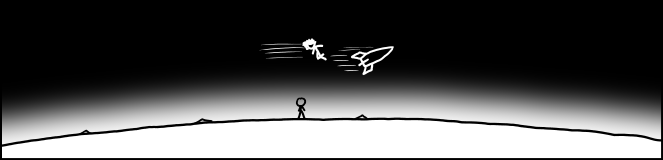
\includegraphics[scale=1.00]{orbit-wide}
  \vfill

  \huge
  \begin{minipage}{0.80\textwidth}
    \setlength\parskip{\medskipamount}
    \vspace{0.3em}
    We will discuss some of the mathematics (and basic physics) involved in
    orbital mechanics. For example: How do we quickly get to the Moon
    without using lots of fuel? Can we save fuel if we have more patience? What
    kind of techniques are involved in touring the solar system? We
    describe some of the methods involved and illustrate these with some videos.

    No prior knowledge is needed. All interested persons are invited to attend.
    There will be cookies.

    \vspace{1em}
    \hfill\small Skript und Übungsblätter: \url{http://pizzaseminar.speicherleck.de/}
  \end{minipage}
\end{center}

\begin{center}
  \Huge
  \vspace*{0.0em}
  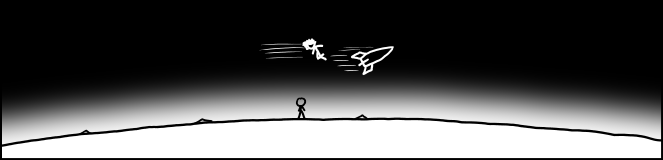
\includegraphics[scale=1.00]{orbit-wide}
  \vspace{0.5em}

  \scalebox{2.5}{Aufgepasst!}
  \scalebox{2.5}{Am Montag gibt es einen}
  \scalebox{2.5}{\textbf{geheimen Bonusvortrag}.}
  \vspace{1em}

  Montag, 1. Dezember 2014, 17:30 Uhr, 2004/L1 \\
  \mbox{\textbf{Otto van Koert: Ein kurzer Einblick in Orbitalmechanik}}

  \Large
  \begin{minipage}{0.80\textwidth}
    \setlength\parskip{\medskipamount}
    \vspace{0.3em}
    Wie kann man ohne viel Treibstoff den Mond erreichen? Wie kann man noch
    mehr Treibstoff einsparen, wenn man es nicht so eilig hat? Welche Techniken
    verwendet man, wenn man durchs Sonnensystem tourt?
    Es werden keine Vorkenntnisse aus Orbitalmechanik vorausgesetzt. Jeder, der
    interessiert ist, kann kommen. Es gibt Kekse und Videos.
  \end{minipage}
\end{center}

\begin{center}
  \Huge
  \vspace*{0.0em}
  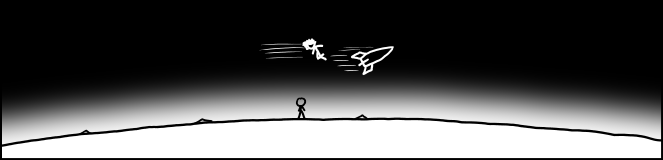
\includegraphics[scale=1.00]{orbit-wide}
  \vspace{0.5em}

  \scalebox{2.4}{Gefährlich!}
  \scalebox{2.4}{\textbf{Verbotener}}\\[0.4em]
  \scalebox{2.5}{\textbf{Geheimvortrag}.}
  \vspace{1em}

  Montag, 1. Dezember 2014, 17:30 Uhr, 2004/L1 \\
  \mbox{\textbf{Otto van Koert: Ein kurzer Einblick in Orbitalmechanik}}

  \Large
  \begin{minipage}{0.80\textwidth}
    \setlength\parskip{\medskipamount}
    \vspace{0.3em}
    Wie kann man ohne viel Treibstoff den Mond erreichen? Wie kann man noch
    mehr Treibstoff einsparen, wenn man es nicht so eilig hat? Welche Techniken
    verwendet man, wenn man durchs Sonnensystem tourt?
    Es werden keine Vorkenntnisse aus Orbitalmechanik vorausgesetzt. Jeder, der
    interessiert ist, kann kommen. Es gibt Kekse und Videos.
  \end{minipage}
\end{center}

\begin{center}
  \Huge
  \vspace*{0.0em}
  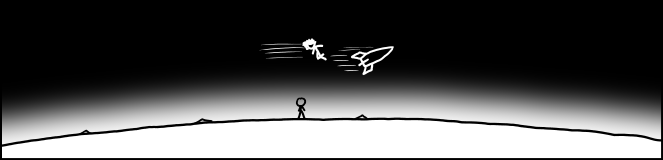
\includegraphics[scale=1.00]{orbit-wide}
  \vspace{0.5em}

  \scalebox{2.4}{Geh da nicht hin!}\\[0.6em]
  \scalebox{2.4}{\textbf{Gefährlicher}}\\[0.6em]
  \scalebox{2.5}{\textbf{Geheimvortrag}.}
  \vspace{1em}

  Montag, 1. Dezember 2014, 17:30 Uhr, 2004/L1 \\
  \mbox{\textbf{Otto van Koert: Ein kurzer Einblick in Orbitalmechanik}}

  \Large
  \begin{minipage}{0.80\textwidth}
    \setlength\parskip{\medskipamount}
    \vspace{0.3em}
    Wie kann man ohne viel Treibstoff den Mond erreichen? Wie kann man noch
    mehr Treibstoff einsparen, wenn man es nicht so eilig hat? Welche Techniken
    verwendet man, wenn man durchs Sonnensystem tourt?
    Es werden keine Vorkenntnisse aus Orbitalmechanik vorausgesetzt. Philipp
    und Ingo laden alle ein, die interessiert sind. Es gibt Kekse und Videos.
  \end{minipage}
\end{center}

\begin{center}
  \Huge
  \vspace*{0.0em}
  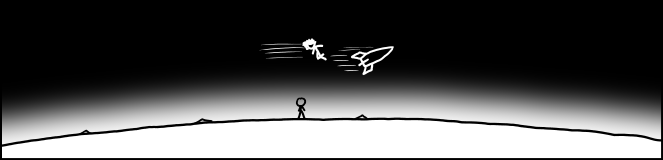
\includegraphics[scale=1.00]{orbit-wide}
  \vspace{0.5em}

  \scalebox{2.5}{Aufgepasst!}\\[0.2em]
  \scalebox{2.5}{Heute Abend gibt es einen}\\[0.2em]
  \scalebox{2.5}{\textbf{geheimen Bonusvortrag}.}
  \vspace{0.7em}

  Montag, 1. Dezember 2014, 17:30 Uhr, 2004/L1 \\
  \mbox{\textbf{Otto van Koert: Ein kurzer Einblick in Orbitalmechanik}}

  \Large
  \begin{minipage}{0.80\textwidth}
    \setlength\parskip{\medskipamount}
    \vspace{0.3em}
    Wie kann man ohne viel Treibstoff den Mond erreichen? Wie kann man noch
    mehr Treibstoff einsparen, wenn man es nicht so eilig hat? Welche Techniken
    verwendet man, wenn man durchs Sonnensystem tourt? Der Vortrag gehört zum
    Pizzaseminar in Mathematik, einem informalen Seminar von Studenten für
    Studenten -- ohne Noten und ohne Prüfer. Es werden keine Vorkenntnisse aus
    Orbitalmechanik oder Homotopischer Algebra~VI vorausgesetzt.
    \textbf{Philipp und Ingo laden alle ein, die interessiert sind.}
    Schau einfach vorbei. Es gibt Kekse und Videos.
  \end{minipage}
\end{center}

\begin{center}
  \Huge
  \vspace*{0.0em}
  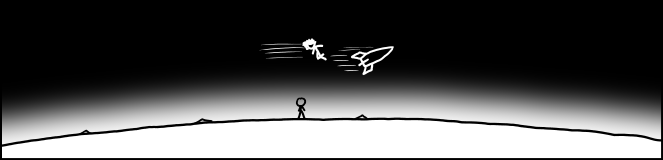
\includegraphics[scale=1.00]{orbit-wide}
  \vspace{0.5em}

  \scalebox{2.4}{Geh da nicht hin!}\\[0.6em]
  \scalebox{2.4}{\textbf{Gefährlicher}}\\[0.6em]
  \scalebox{2.5}{\textbf{Geheimvortrag}.}
  \vspace{1em}

  Montag, 1. Dezember 2014, 17:30 Uhr, 2004/L1 \\
  \mbox{\textbf{Otto van Koert: Ein kurzer Einblick in Orbitalmechanik}}

  \Large
  \begin{minipage}{0.80\textwidth}
    \setlength\parskip{\medskipamount}
    \vspace{0.3em}
    Wie kann man ohne viel Treibstoff den Mond erreichen? Wie kann man noch
    mehr Treibstoff einsparen, wenn man es nicht so eilig hat? Welche Techniken
    verwendet man, wenn man durchs Sonnensystem tourt? Der Vortrag gehört zum
    Pizzaseminar in Mathematik, einem informalen Seminar von Studenten für
    Studenten -- ohne Noten und ohne Prüfer. Es werden keine Vorkenntnisse aus
    Orbitalmechanik oder Homotopischer Algebra~VI vorausgesetzt.
    \textbf{Philipp und Ingo laden alle ein, die interessiert sind.}
    Schau einfach vorbei. Es gibt Kekse und Videos.
  \end{minipage}
\end{center}

\end{document}
